\chapter{Seznam videí}
Tato příloha obsahuje kompletní seznam videí vzniklých v rámci projektu P3D vč. odkazů rozdělených dle jednotlivých témat. \newline
\noindent\It{Pozn.: při kliknutí na odkaz budete přesněrování na stránku korespondujícího videa (pouze v digitální verzi)}.

\section{Instalace a zprovoznění SolidWorks SDK}
\href{https://aka.parallaxproduction.cz/instalaceSDK}{Instalace a první spuštění SolidWorks SDK 2020/2021 (aka.parallaxproduction.cz/instSDK)} \newline
\href{https://aka.parallaxproduction.cz/sablony}{Instalace šablon a knihoven norm. dílů ze Sokolské (aka.parallaxproduction.cz/sablony)} \newline
\href{https://aka.parallaxproduction.cz/realview}{Aktivace Realview na necertifikované grafické kartě (aka.parallaxproduction.cz/realview)} \newline

\section{Základy modelování}
\href{https://aka.parallaxproduction.cz/jednoducha-pruzina}{Jednoduchá pružina (aka.parallaxproduction.cz/jednoducha-pruzina)} \newline
\href{https://aka.parallaxproduction.cz/j-ozubene-kolo}{Ozubené kolo s přímým čelním ozubením (aka.parallaxproduction.cz/j-ozubene-kolo)} \newline
\href{https://aka.parallaxproduction.cz/vyk-oz-kolo}{Ozubené kolo pro výkres - obálka (aka.parallaxproduction.cz/vyk-oz-kolo)} \newline
\href{https://aka.parallaxproduction.cz/jednorad-r-kolo}{Jednořadé řetězové kolo (aka.parallaxproduction.cz/jednorad-r-kolo)} \newline
\href{https://aka.parallaxproduction.cz/perodrazka-naboj}{Drážka pro pero v náboji (aka.parallaxproduction.cz/perodrazka-naboj)} \newline

\section{Výkresová dokumentace}


\section{Práce se sestavami}


\chapter{Obrazové přílohy}

%\begin{figure}[h]
%    \centering
%    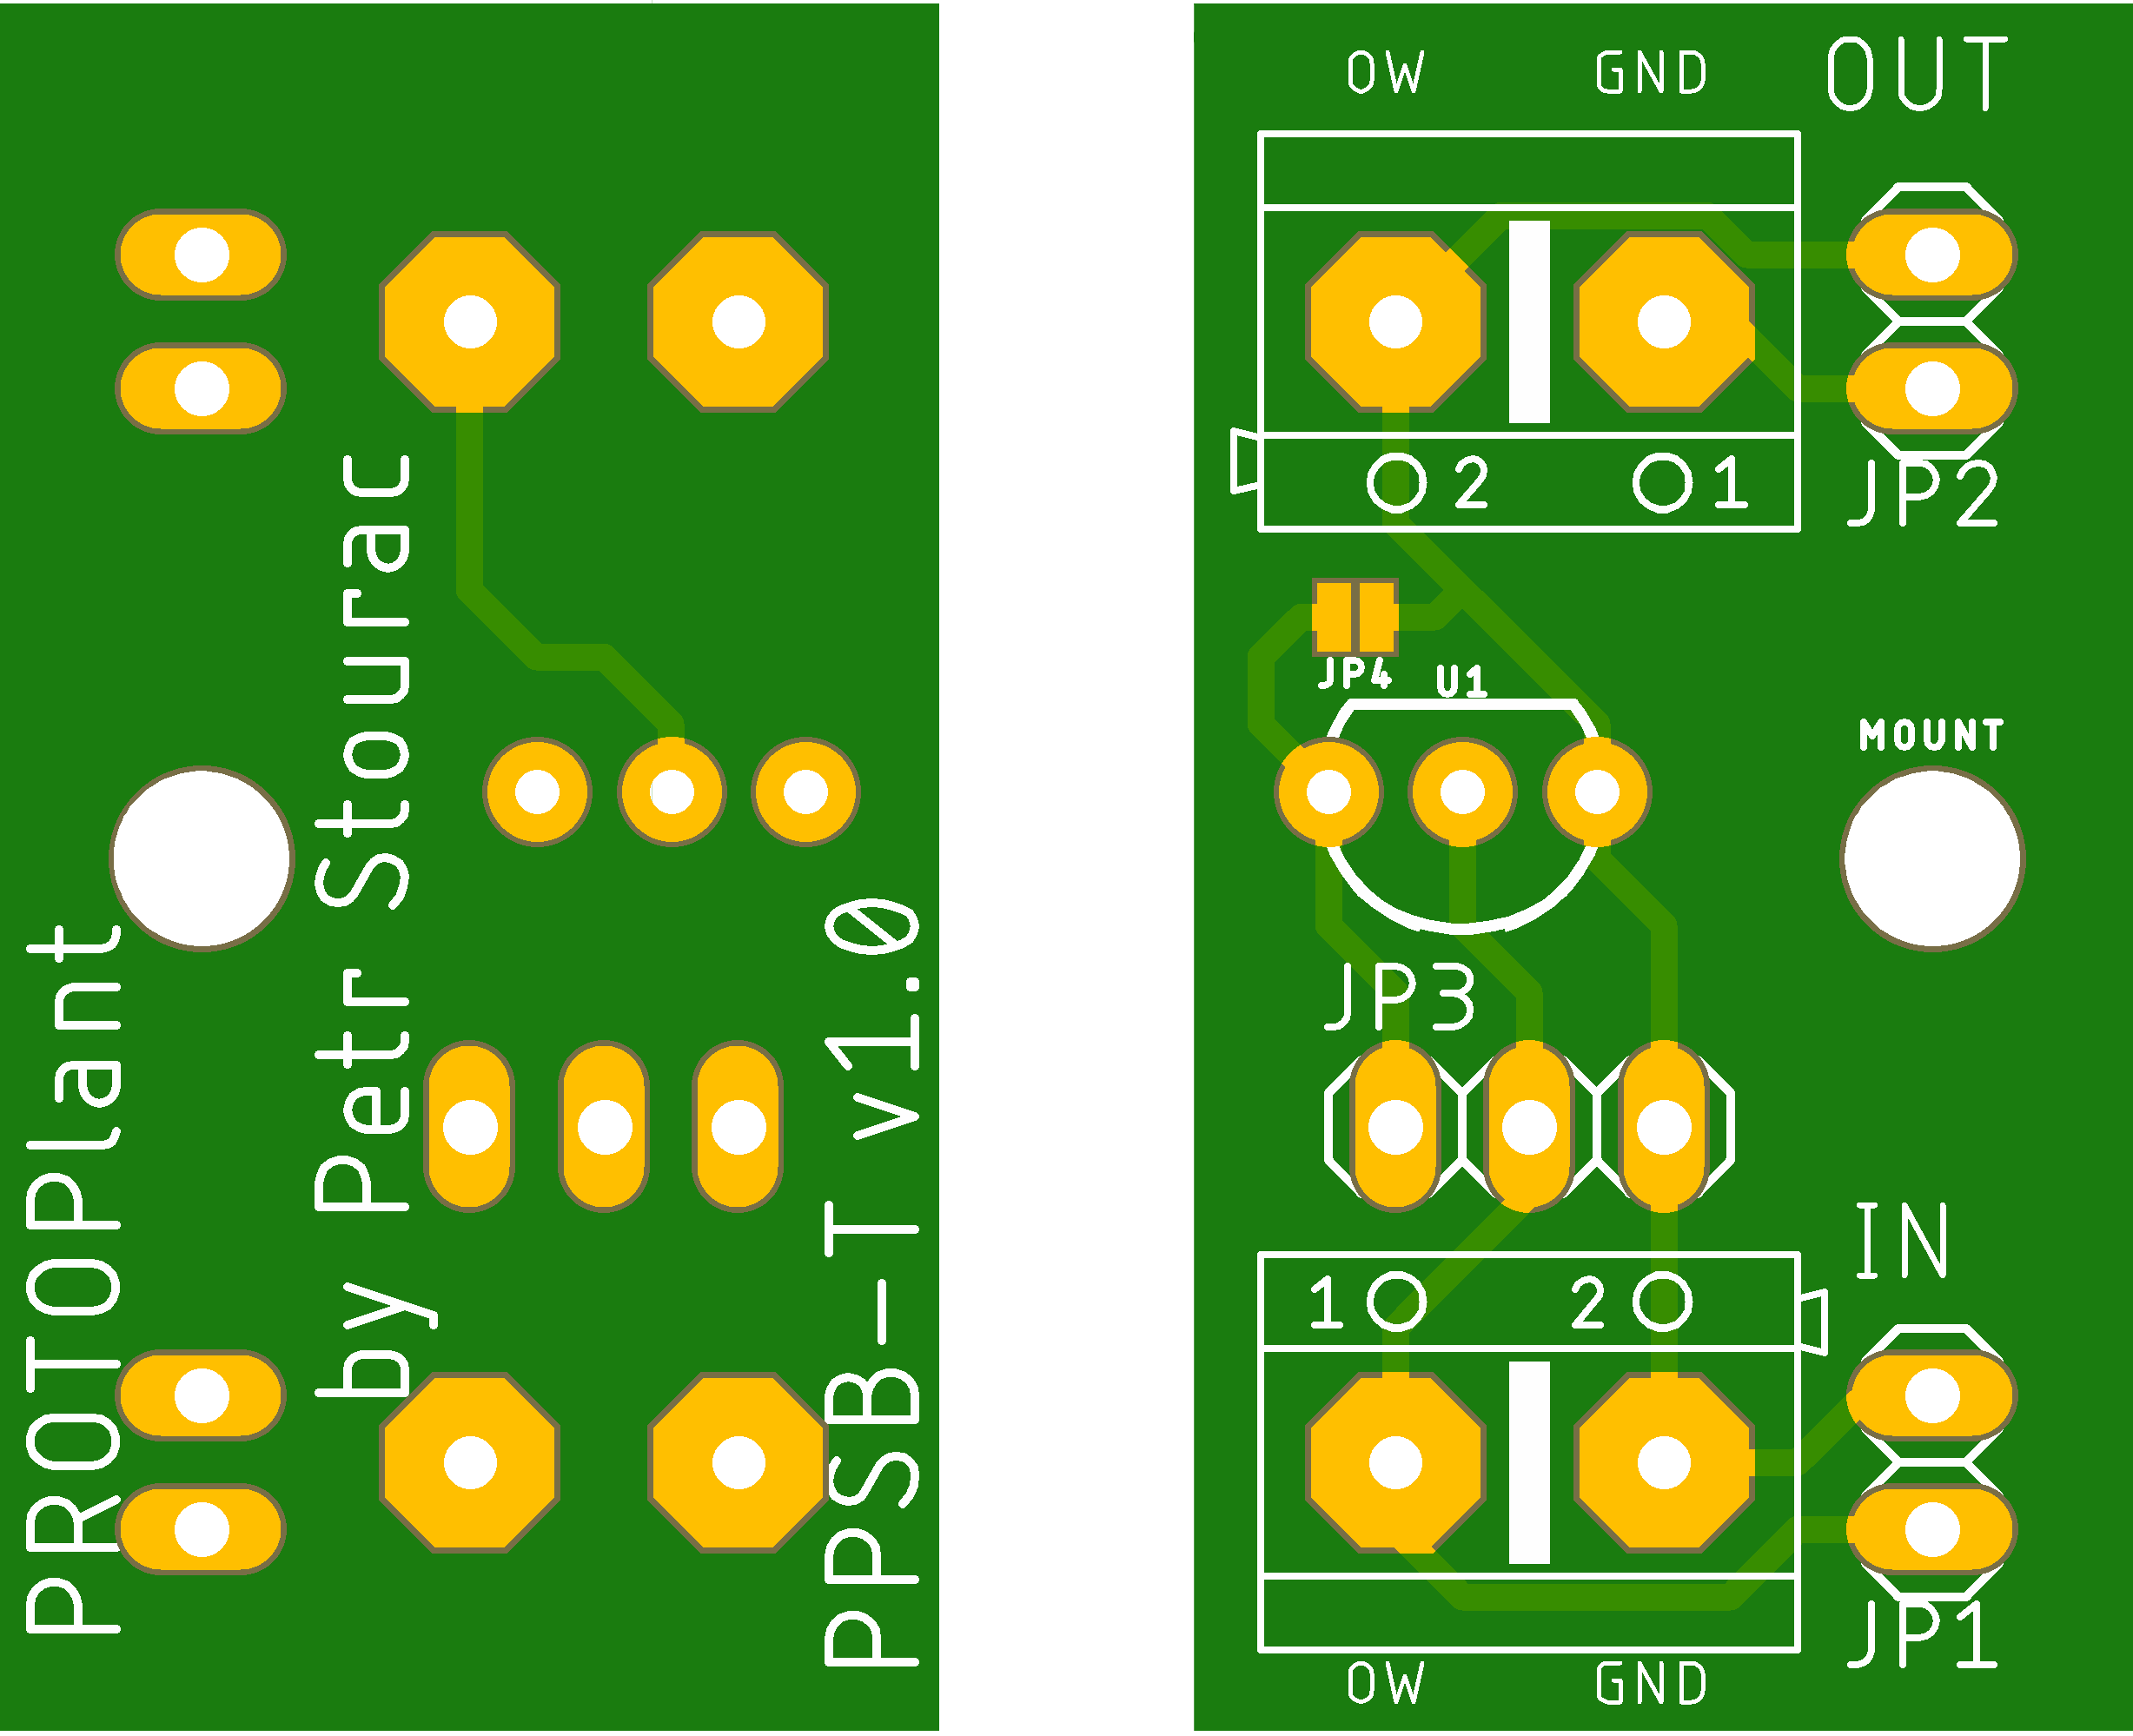
\includegraphics[width=0.85\textwidth]{img/ToBeRemoved/PPSB-T_BOTH.png}
%    \caption{Vizualizace PPSB-T (horní strana vpravo, dolní vlevo).}
%    \label{fig:PPSB-T_VISUAL}
%\end{figure}